\subsection{Log Data Analysis}
\label{log-data-analysis}

Log data collection involves gathering information from various sources like endpoints, applications, and network devices. This data is essential for monitoring system activities and identifying potential security threats. Log data analysis, on the other hand, is the process of examining this collected data to extract useful information and identify patterns or anomalies.

Wazuh collects, analyzes, and stores logs from endpoints, network devices, and applications. The Wazuh agent, running on a monitored endpoint, collects and forwards system and application logs to the Wazuh server for analysis. Additionally, it is possible to send log messages to the Wazuh server via syslog, or third-party API integrations.

\subsubsection{How it works}
Wazuh uses the \texttt{Logcollector} module to collect logs from monitored endpoints, applications, and network devices. The Wazuh server then analyzes the collected logs in real-time using decoders and rules. Wazuh extracts relevant information from the logs and maps them to appropriate fields using decoders. The \texttt{Analysisd} module in the Wazuh server evaluates the decoded logs against rules and records all alerts in \texttt{/var/ossec/logs/alerts/alerts.log} and \texttt{/var/ossec/logs/alerts/alerts.json} files.

The Wazuh server also receives \texttt{syslog} messages from devices that do not support the installation of Wazuh agents, ensuring seamless integration and coverage across the entire network environment.

\begin{figure} [H]
\centering
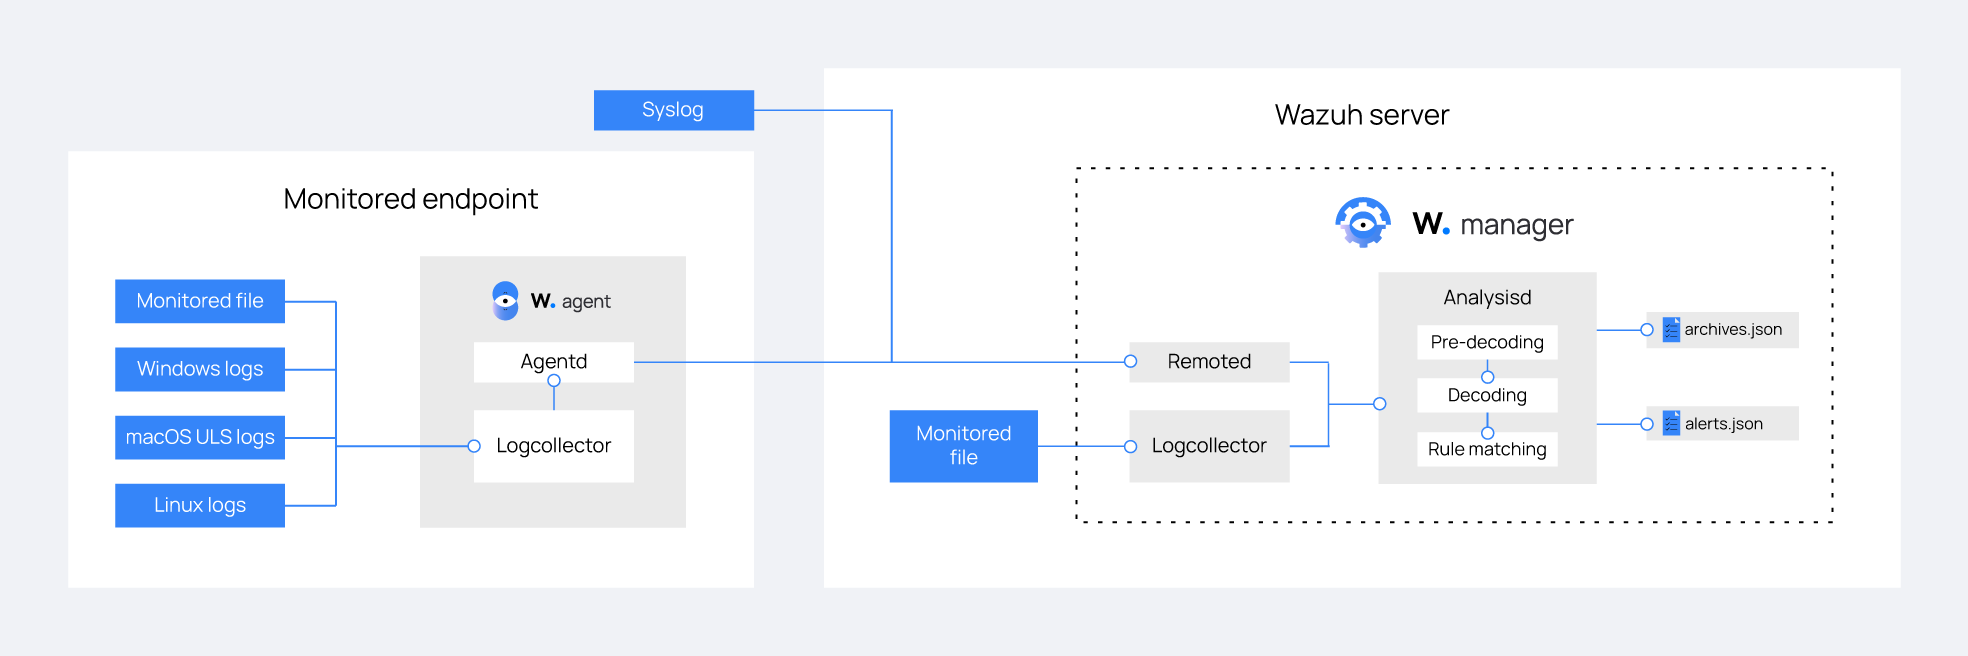
\includegraphics[width=\textwidth]{images/log-data.png}
\caption{The flow of log data collection and analysis in Wazuh}
\label{fig:wazuhlogflow}
\end{figure}

The log data collection process consists of 3 essential phases:
\begin{itemize}
    \item \textbf{Pre-decoding Phase: } This initial stage involves the preliminary processing of collected logs. Here, generic information such as timestamp, hostname, and log source is extracted. The purpose of pre-decoding is to standardize the log format, which enables more detailed analysis.
    \item \textbf{Decoding Phase: } In this critical phase, the pre-decoded log data is converted to a more structured and readable format. The Wazuh decoders parse each log to extract detailed information and map it to specific fields. This process involves processing the log content to identify and categorize elements such as user IDs, source IP addresses, and error codes. The decoding phase transforms raw data into structured information, making precise security monitoring possible from log data analysis.
    \item \textbf{Rule Matching Phase: } Following decoding, the logs are matched against a comprehensive set of predefined rules in the \texttt{Analysisd} module. This phase is fundamental to identifying security incidents or policy violations. Each log is scrutinized, and if certain criteria are met, an alert is generated. This matching process not only identifies potential threats but also categorizes them based on severity, relevance, and type, enabling targeted response mechanisms and efficient threat mitigation.
\end{itemize}


By default, the Wazuh server retains logs and does not delete them automatically. However, the user can choose when to manually or automatically delete these logs according to their legal and regulatory requirements.

In addition to alert logs, Wazuh stores all collected logs in dedicated archive log files, specifically \texttt{archives.log} and \texttt{archives.json} in \texttt{/var/ossec/logs/archives/}. These archive log files comprehensively capture all logs, including those that do not trigger any alerts. This feature ensures a comprehensive record of all system activities for future reference and analysis.

\subsubsection{Configuration}

Wazuh supports two primary methods of log data collection.

\paragraph{Using Syslog}
The Wazuh server can be configured to listen for incoming syslog messages on predefined ports, enabling support for devices without support for Wazuh Agent. The primary configuration adjustments are made using the \texttt{ossec.conf} file located on the server.

\subparagraph{Listening for Syslog Messages}
The essential part of the configuration involves defining a \texttt{<remote>} block within the \texttt{ossec.conf} file of the Wazuh server. An example configuration is as follows:

\begin{minted}{xml}
<remote>
    <connection>syslog</connection>
    <port>514</port>
    <protocol>tcp</protocol>
    <allowed-ips>192.168.2.15/24</allowed-ips>
    <local_ip>192.168.2.10</local_ip>
</remote>
\end{minted}

In this context:
\begin{itemize}
    \item \texttt{<connection>} defines the connection type.
    \item \texttt{<port>} specifies the listening port.
    \item \texttt{<protocol>} indicates the communication protocol.
    \item \texttt{<allowed-ips>} designates permitted sender IP addresses.
    \item \texttt{<local\_ip>} is the server's IP address that will listen for log messages.
\end{itemize}

For changes to take effect, the Wazuh manager requires a restart. This is typically performed via the command:

\begin{minted}{bash}
systemctl restart wazuh-manager
\end{minted}

\paragraph{Using Wazuh Agent}
On devices where Wazuh Agent can be installed, log files can be monitored by simply changing the agent configuration.

\subparagraph{Monitoring Basic Log Files}
Configuration for monitoring basic log files involves inserting the \texttt{localfile} XML blocks into the \texttt{ossec.conf} file of the Wazuh agent. The following is an illustrative example:

\begin{minted}{xml}
<localfile>
    <location>/path/to/log/file.log</location>
    <log_format>syslog</log_format>
</localfile>
\end{minted}

\subparagraph{Monitoring Date-based Log Files}
To adapt to dynamic file naming based on dates, the configuration supports strftime format. An example configuration is shown below:

\begin{minted}{xml}
<localfile>
    <location>/path/to/log/file-%y-%m-%d.log</location>
    <log_format>syslog</log_format>
</localfile>
\end{minted}

\subparagraph{Monitoring Using Wildcard Patterns}
Wazuh allows for the use of wildcard patterns to monitor multiple log files within a directory. An example of such a configuration is:

\begin{minted}{xml}
<localfile>
    <location>/path/to/logs/file*.log</location>
    <log_format>syslog</log_format>
</localfile>
\end{minted}

\subparagraph{Utilizing Environment Variables in Log Monitoring}
Particularly on Windows, Wazuh configurations can incorporate environment variables within log file paths, adding flexibility to the monitoring setup:

\begin{minted}{xml}
<localfile>
    <location>%WINDIR%\Logs\CustomLog.log</location>
    <log_format>syslog</log_format>
</localfile>
\end{minted}


\subsubsection{Simulation}
We demonstrate the following two use-cases of Log Data Analysis.
\paragraph{Linux Log Data Analysis using \texttt{rsyslog}}
In this use case, we configure a \texttt{Ubuntu 20.04.6} endpoint to forward logs using rsyslog to the Wazuh server for analysis. On the \texttt{Ubuntu 20.04.6} endpoint, we create and delete the user account Alice. Wazuh has default rules that generate alerts for the creation and deletion of user accounts.

\subparagraph{Ubuntu endpoint}
\begin{enumerate}
    \item We edit the \texttt{/etc/rsyslog.conf} file and add the following configuration
    \begin{figure} [H]
    \centering
    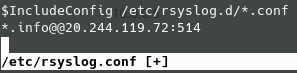
\includegraphics[width=0.4\textwidth]{images/log-data/1.png}
    \caption{\texttt{rsyslog} configuration}
    \end{figure}
    Here \texttt{20.244.119.72} is the IP address of our Wazuh Server.
    \item We restart the \texttt{rsyslog} service to apply changes.
    \begin{figure} [H]
    \centering
    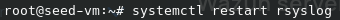
\includegraphics[width=0.5\textwidth]{images/log-data/2.png}
    \caption{Restart \texttt{rsyslog}}
    \end{figure}
\end{enumerate}

\subparagraph{Wazuh server}
\begin{enumerate}
    \item We edit the \texttt{/var/ossec/etc/ossec.conf} file and add the following configuration in between the \texttt{<ossec\_config>} tags:
    \begin{figure} [H]
    \centering
    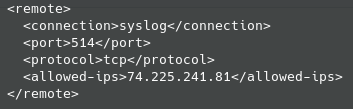
\includegraphics[width=0.5\textwidth]{images/log-data/3.png}
    \caption{Wazuh server configuration}
    \end{figure}
    Here \texttt{74.225.241.81} is the IP address of the Ubuntu endpoint.
    
    \item We restart Wazuh Manager for the configuration to take effect.
\end{enumerate}

We test the configuration in the next sub-section. 

\paragraph{Windows Log Data Analysis using Wazuh Agent}
In this use case, we configure a \texttt{Windows 11} device running Wazuh Agent for log data analysis. On \texttt{Windows 11} we install the software Dr. Memory. On the Wazuh Server we create rules for generating alerts when new software is installed.

\subparagraph{Windows endpoint}
\begin{enumerate}
    \item We edit the Wazuh Agent configuration file at \texttt{C:/Program Files (x86)/ossec-agent/ossec.conf} and add the following block inside the \texttt{<ossec\_config>} tag.
    \begin{figure} [H]
    \centering
    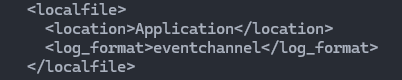
\includegraphics[width=0.8\textwidth]{images/log-data/9.png}
    \caption{Wazuh Agent configuration}
    \end{figure}
    \item We restart Wazuh Agent for the change to apply.
\end{enumerate}

\subparagraph{Wazuh server}
\begin{enumerate}
    \item We create or modify the following rule at \\ \texttt{/var/ossec/ruleset/rules/0585-win-application\_rules.xml} to generate alerts when new application is installed.
    \begin{figure} [H]
    \centering
    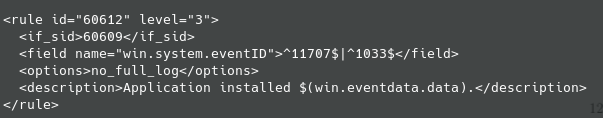
\includegraphics[width=0.8\textwidth]{images/log-data/10.png}
    \caption{Wazuh server configuration}
    \end{figure}
    \item We restart Wazuh Manager for the configuration to take effect.
\end{enumerate}

\subsubsection{Dashboard Update}
\paragraph{Linux Log Data Analysis using \texttt{rsyslog}}
\begin{enumerate}
    \item We add the new user \texttt{Alice}
    \begin{figure} [H]
    \centering
    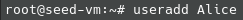
\includegraphics[width=0.4\textwidth]{images/log-data/7.png}
    \caption{Adding new user}
    \end{figure}
    \item We delete the user \texttt{Alice}
    \begin{figure} [H]
    \centering
    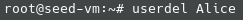
\includegraphics[width=0.4\textwidth]{images/log-data/8.png}
    \caption{Deleting the new user}
    \end{figure}
    \item We navigate to the \texttt{Modules > Security events} tab in the Wazuh Dashboards to view the alerts. 
    \begin{figure} [H]
    \centering
    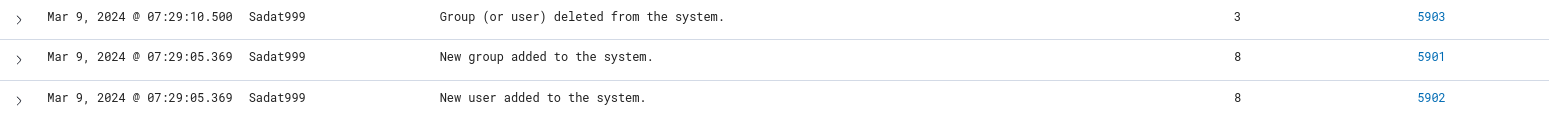
\includegraphics[width=\textwidth]{images/log-data/4.png}
    \caption{Alerts for user/group creation and deletion}
    \end{figure}
    \item We expand the alert to see more details.
    \begin{figure} [H]
    \centering
    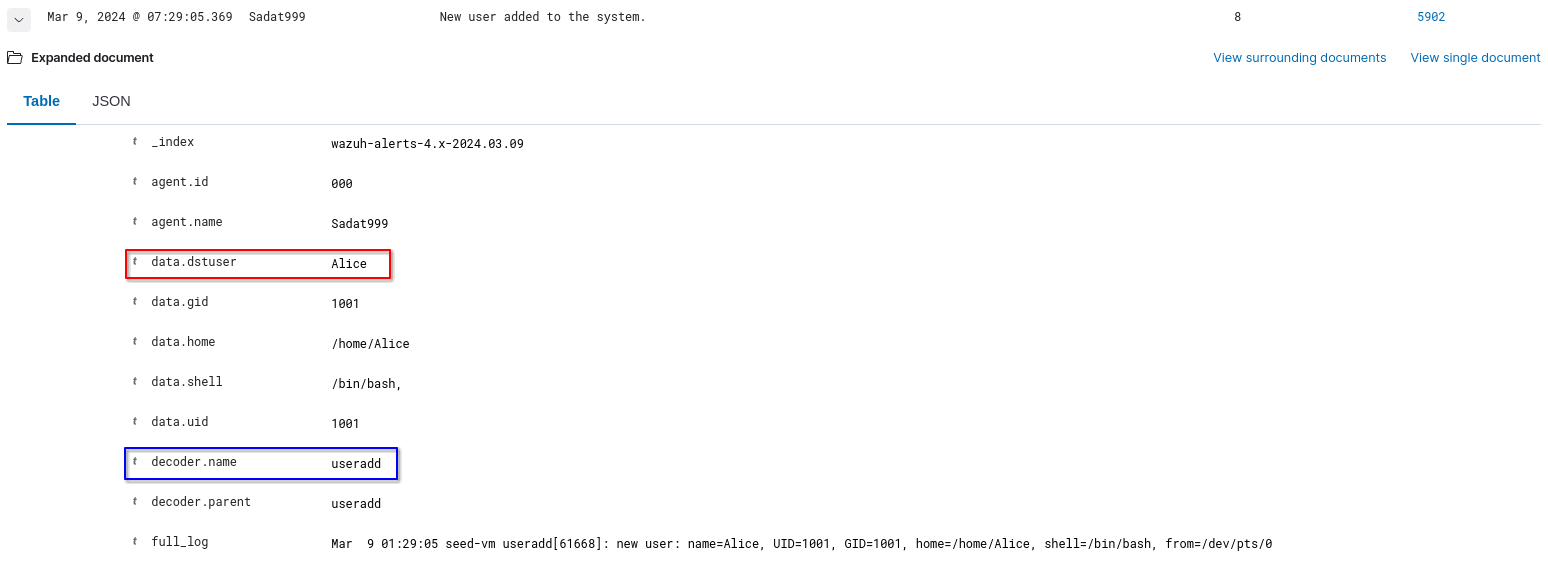
\includegraphics[width=0.5\textwidth]{images/log-data/5.png}
    \caption{The name of the new user (red), the decoder used to process the log (blue)}
    \end{figure}
    \begin{figure} [H]
    \centering
    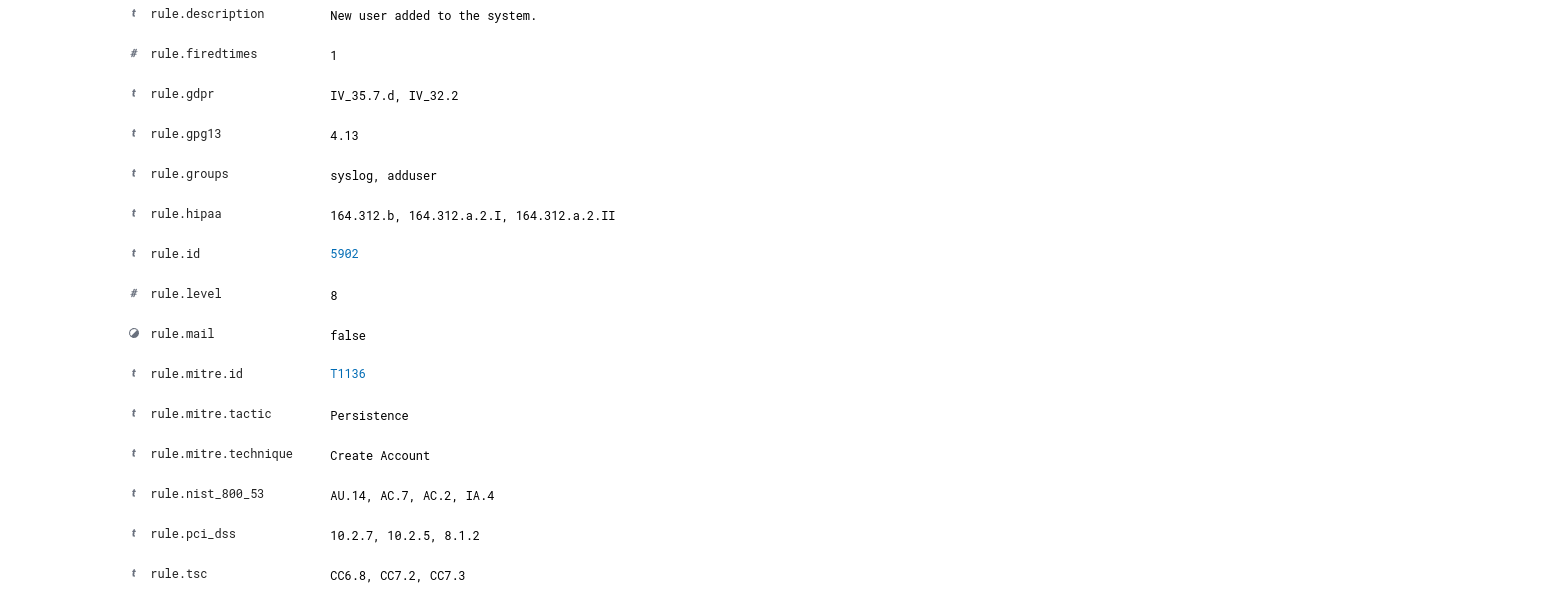
\includegraphics[width=\textwidth]{images/log-data/6.png}
    \caption{Details of the rule used to generate this alert}
    \end{figure}
\end{enumerate}


\paragraph{Windows Log Data Analysis using Wazuh Agent}
\begin{enumerate}
    \item We download the software \href{https://drmemory.org}{Dr. Memory}.
    \item We install the application on the \texttt{Windows 11} machine.
    \begin{figure} [H]
    \centering
    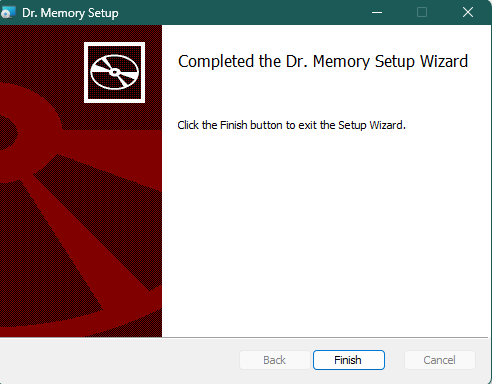
\includegraphics[width=0.4\textwidth]{images/log-data/11.png}
    \caption{Installation of Dr. Memory}
    \end{figure}
    \item We navigate to the \texttt{Modules > Security events} tab in the Wazuh Dashboards to view the alert. 
    \begin{figure} [H]
    \centering
    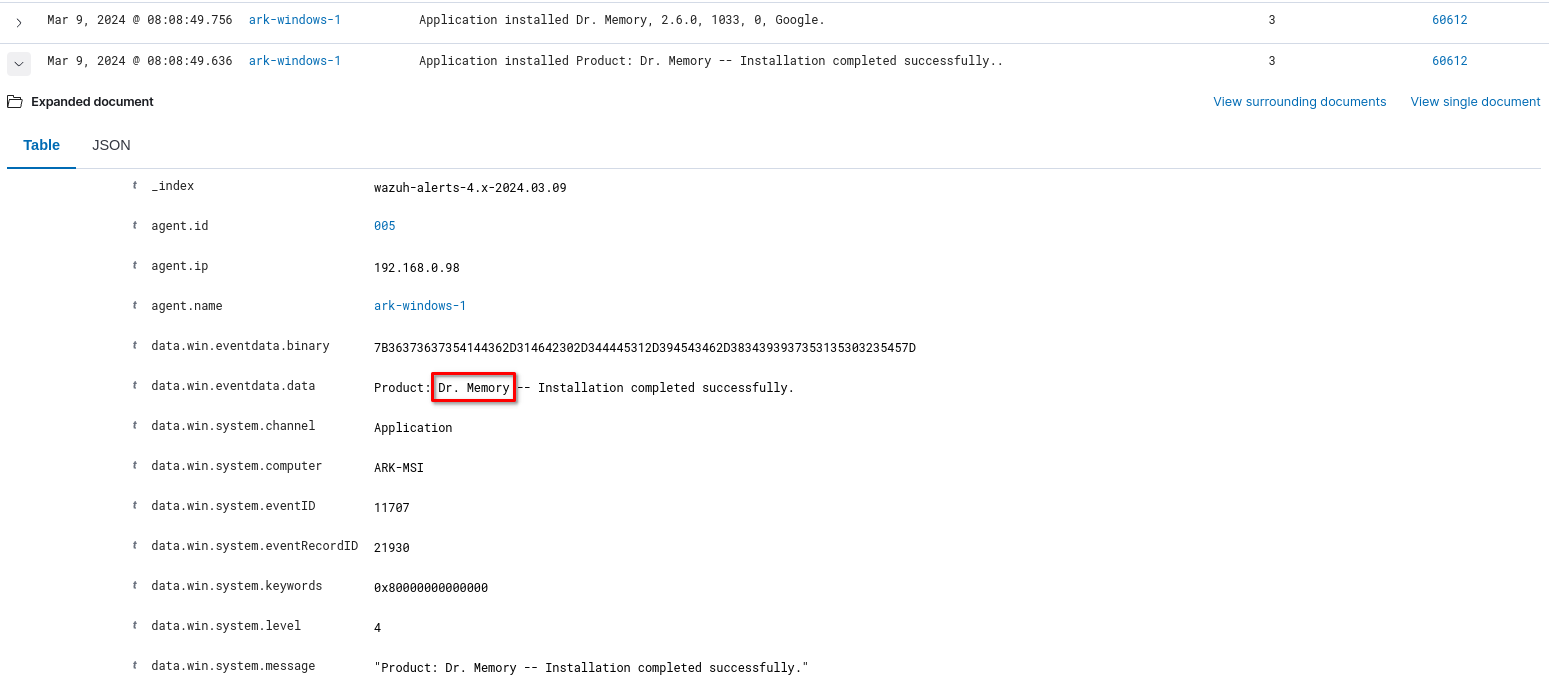
\includegraphics[width=0.4\textwidth]{images/log-data/12.png}
    \caption{Alert for new software installation}
    \end{figure}
\end{enumerate}
